\begin{table}[t]
\centering\small
\resizebox{\columnwidth}{!}{\begin{tabular}{lcccc}
\toprule
 & \multicolumn{2}{c}{IMDB (text, $K{=}10$)} & \multicolumn{2}{c}{Heart (tabular, $K{=}5$)} \\
\cmidrule(lr){2-3}\cmidrule(lr){4-5}
 & Sparse LR & DT & Sparse LR & DT \\
\midrule
Random & 11.8 & 11.0 & 38.2 & 39.0 \\
Parzen & 45.7 & 17.9 & 40.7 & 45.3 \\
Greedy & 49.6 & 36.2 & 28.2 & 28.2 \\
LIME & 81.4 & 95.2 & 97.4 & 66.4 \\
\midrule
Mean $|$gold$|$ & 3.3 & 1.6 & 4.8 & 4.4 \\
\bottomrule
\end{tabular}
}
\caption{Faithfulness on new data: recall (\%) of gold features. Same protocol as Table~\ref{tab:recallrepl}. Heart uses $K{=}5$ of 13 features, so Random's expected recall is about 38\%.}
\label{tab:recallnew}
\end{table}

\begin{table*}[t]
\centering\small
\resizebox{0.8\textwidth}{!}{\begin{tabular}{lcccccccc}
\toprule
 & \multicolumn{4}{c}{IMDB} & \multicolumn{4}{c}{Heart} \\
\cmidrule(lr){2-5}\cmidrule(lr){6-9}
 & LR & NN & RF & SVM & LR & NN & RF & SVM \\
\midrule
Random & 12.8 & 12.6 & 12.9 & 12.8 & 32.3 & 31.3 & 32.0 & 32.1 \\
Parzen & 85.7 & 85.5 & 90.9 & 90.5 & 93.3 & 91.5 & 94.0 & 94.9 \\
Greedy & 48.0 & 45.9 & 45.4 & 48.8 & 66.9 & 60.2 & 65.0 & 60.5 \\
LIME & 95.3 & 92.9 & 97.8 & 95.2 & 87.7 & 86.7 & 88.9 & 87.4 \\
\midrule
Test acc. & 82.5 & 57.8 & 79.0 & 81.5 & 83.8 & 82.5 & 83.8 & 83.5 \\
Flipped & 12.1\% & 25.2\% & 12.3\% & 12.1\% & 9.9\% & 14.6\% & 9.1\% & 9.0\% \\
\bottomrule
\end{tabular}
}
\caption{Trust on new data: F1 (\%) of the trustworthy class, same protocol as Table~\ref{tab:trustrepl}. Heart: 3 of 13 features untrustworthy, $K{=}5$, 297 patients via 5-fold cross-fitting. All LIME--baseline differences are significant ($p<10^{-4}$). On Heart, Parzen is significantly \emph{better} than LIME.}
\label{tab:trustnew}
\end{table*}

\begin{figure*}[t]
\centering
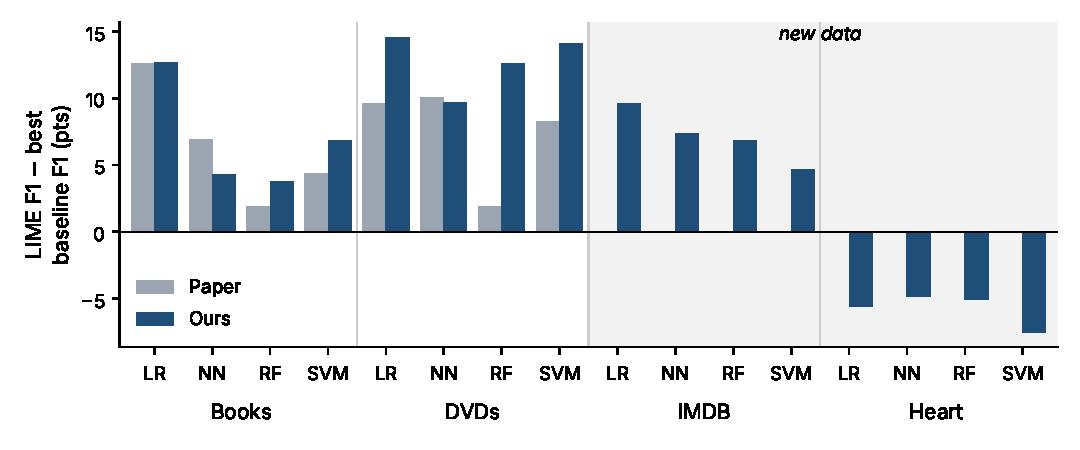
\includegraphics[width=0.85\textwidth]{generated/fig_trust_margin.pdf}
\caption{LIME's margin over the best of the three baselines in the trust experiment (F1 points). Grey bars are the paper's Table~1, dark bars are ours. The margin is preserved in every replicated setting and on IMDB, and turns negative on tabular Heart data.}
\label{fig:margin}
\end{figure*}

\subsection{Simulated-user experiments}
\paragraph{New text domain (IMDB).} LIME generalises to movie reviews. In the trust experiment its F1 is \IMDBLimeTrustRange{} (Table~\ref{tab:trustnew}), which is within the range of the replication (\ReplTrustRange{}), and the method ordering is unchanged. Parzen (\IMDBParzenTrustRange{}) and Greedy behave as on Books/DVDs. For faithfulness (Table~\ref{tab:recallnew}), LIME recovers \IMDBTreeRecall{}\% of the tree's gold words, close to Books and DVDs (94.1 and 96.5). For the sparse LR it recovers \IMDBLRRecall{}\%, below Books and DVDs (85.1 and 90.9). IMDB reviews have about 147 distinct words, against 85 in the authors' Books/DVDs files, so each document has more candidate words competing for the same $K{=}10$ slots, and the sampler drops a smaller fraction of the relevant words in each perturbation. Even so, LIME's recall is 32 points above the next-best explainer.

\paragraph{New modality (Heart Disease).} The tabular results diverge from the paper's conclusions in two ways. \emph{Faithfulness:} LIME recovers \HeartLRRecall{}\% of the sparse LR's gold features but only \HeartTreeRecall{}\% of the decision tree's, against 94.1--96.5\% on the three text datasets. The tabular explainer discretises continuous features into training-set quartiles and perturbs by resampling bins, so a split in the tree at, say, \texttt{oldpeak}\,${\le}\,0.7$ can fall inside a quartile. Perturbations then rarely cross the threshold and the feature looks locally irrelevant. On text there is no such mismatch, because removing a word is exactly the operation a word-presence split tests. \emph{Trust:} Parzen (\HeartParzenTrustRange{}) significantly outperforms LIME (\HeartLimeTrustRange{}) for all four classifiers (Figure~\ref{fig:margin}). Table~\ref{tab:prf} shows why: LIME's precision stays high (92--96\%) but its recall falls to 82--84\%, so it distrusts too many trustworthy predictions. LIME's interpretable features for tabular data mean ``the patient is in bin $b$'', and the trust rule removes a feature by subtracting its weight, which is equivalent to moving the patient \emph{out of} that bin. The oracle instead resets the feature to its training median or mode, and for 45\% of (patient, feature) pairs that leaves the patient in the same bin (37\% exactly unchanged, e.g.\ \emph{sex = male} is also the mode). LIME therefore predicts a change where none happens. Our Parzen adaptation measures the change towards exactly that baseline, so part of its advantage comes from the evaluation design. That is itself the finding: LIME's tabular explanations describe deviation from the training distribution, not from a particular reference value, and a user who reads ``removing this feature'' literally will be misled. The paper's text-only evaluation could not reveal this.

\paragraph{Against the replication.} The new data agrees with the replication on text and disagrees on tables. On IMDB, LIME is again the best explainer in every setting, its trust F1 (\IMDBLimeTrustRange{}) lies inside the replicated range (\ReplTrustRange{}), and its recall of the tree's features (\IMDBTreeRecall{}\%) matches Books and DVDs. On Heart Disease, two of the replication's conclusions fail: LIME's recall of the tree's features falls to \HeartTreeRecall{}\%, and Parzen, never better than LIME in any replicated setting, beats it in all four trust settings.

\subsection{Human and LLM trust judgements}
\label{sec:humanres}
% Numbers come from report/generated/annotation_macros.tex (src/analyze_annotations.py).
\paragraph{Agreement between people.} All three annotators completed all 60 items (one Q2 answer was left blank). Inter-annotator agreement on trust is Krippendorff's $\alpha$\,=\,\AlphaTrust{} (ordinal), and pairwise quadratic-weighted $\kappa$ ranges over \PairQWKRange{}, i.e.\ moderate to substantial agreement. Agreement on whether an explanation ``makes sense'' is lower ($\alpha$\,=\,\AlphaSense{}, nominal), so judging the medical plausibility of a reason is harder for non-experts than giving an overall trust rating. Annotator C was the most sceptical, and the mean trust over all ratings is \MeanTrustHuman{} on the 1--5 scale.

\paragraph{Do explanations help people spot wrong predictions?} Correct predictions received a mean human trust of \TrustCorrect{}, and incorrect ones \TrustIncorrect{} (Mann--Whitney $p$\,=\,\PTrustMW{}). Averaged trust separates correct from incorrect predictions with ROC AUC \AUCHuman{} (95\% bootstrap CI \AUCLo{}--\AUCHi{}; 0.5 is chance), and explanations were judged to make sense for \SenseCorrect{} of correct but only \SenseIncorrect{} of incorrect predictions. On the face of it this supports the paper's claim. However, human trust correlates almost perfectly with the model confidence printed next to each prediction (Spearman $\rho$\,=\,\RhoHumanConf{}), and confidence \emph{alone} separates correct from incorrect predictions just as well (AUC \AUCConf{}). Once confidence is regressed out, the remaining variation in human trust carries no signal about correctness (AUC \AUCResid{}, $p$\,=\,\PResid{}), and trust correlates only weakly with LIME's local fidelity ($\rho$\,=\,\RhoHumanRtwo{}). Our raters could tell good predictions from bad, but we find no evidence that LIME's explanations contributed beyond the confidence score. Because every item showed both, the design cannot rule out a smaller effect; an explanation-versus-no-explanation condition would be needed to measure it (\S\ref{sec:concl}).

\paragraph{LLM-as-judge.} The judge (\LLMModel{}, three repeats) is almost perfectly self-consistent ($\alpha$\,=\,\LLMSelfAlpha{}), and it ranks items much as people do: Spearman $\rho$\,=\,\LLMvsHumanRho{} with the mean human rating, and quadratic-weighted $\kappa$\,=\,\LLMvsHumanQWK{} with the human median. That is within the range of agreement between the humans themselves (\PairQWKRange{}). As a rater, however, it is systematically lenient. Its mean trust is \MeanTrustLLM{} against \MeanTrustHuman{} for humans, it never gave a rating below 3 (humans gave 1--2 in 18\% of ratings), and it answered ``Yes, the explanation makes sense'' for all 180 judgements, against 63\% for humans. Agreement with the human Q2 majority is therefore $\kappa$\,=\,\LLMvsHumanSenseKappa{} by construction, and adding the judge as a fourth rater \emph{lowers} the group's $\alpha$ from \AlphaTrust{} to \AlphaTrustWithLLM{}. Its trust separates correct from incorrect predictions less well than the humans' (AUC \AUCLLM{} vs.\ \AUCHuman{}; mean \LLMTrustCorrect{} vs.\ \LLMTrustIncorrect{}). Like the humans, it mostly follows the displayed confidence ($\rho$\,=\,\RhoLLMConf{}), and beyond confidence it carries no signal (AUC \AUCLLMResid{}). Its stated reasons are generic (e.g.\ ``the explanation aligns with the patient's clinical attributes that are known risk factors''). This confirms the risk anticipated in our proposal: an LLM judge accepts fluent, plausible-sounding explanations rather than checking them. It is a cheap, reproducible proxy for the \emph{ranking} of human trust, but not a substitute for human judgement of whether an explanation is sound.


\paragraph{How this evaluation differs from the replication.} The simulated-user experiments define an untrustworthy prediction as one that depends on randomly designated ``untrustworthy'' features, and the simulated user applies a fixed rule to the explanation. In the annotation study, ground truth is whether the prediction is actually correct, and the users are people (or an LLM) who bring their own prior beliefs about heart disease. The paper's human studies were closer to this but used text classifiers and Mechanical Turk workers. Ours applies the question to tabular clinical data, the setting in which the simulated results above suggest LIME is least reliable.
